%% ============================================================
%%  INFORME FINAL PIB - Proyecto de Ingeniería Biomédica 2026
%%  Escuela de Ingeniería Civil Biomédica - Universidad de Valparaíso
%%  Autor: Cristian Raúl Salgado Torres
%%  Tema:  Machine Learning causal en Resonancia Magnética Funcional
%% ============================================================

\documentclass[12pt,letterpaper]{article}

%% ------------------------------------------------------------
%% PAQUETES
%% ------------------------------------------------------------
\usepackage[spanish,es-nodecimaldot]{babel}
\shorthandoff{<>} % evita conflicto de babel ("<" ">" activos) con TikZ (>=Latex)
\usepackage{iftex}
\ifPDFTeX
  \usepackage[utf8]{inputenc}
  \usepackage[T1]{fontenc}
  \usepackage{mathptmx}
  \renewcommand{\sfdefault}{ptm}
\else
  \usepackage{fontspec}
  \setmainfont{Times New Roman}
  \setsansfont{Times New Roman}
\fi
\usepackage{geometry}
\usepackage{graphicx}
\usepackage{multicol}
\usepackage{titlesec}
\usepackage{tocloft} % personalización de Tabla de contenidos
\usepackage{fancyhdr}
\usepackage{parskip}
\usepackage{booktabs}
\usepackage{array}
\usepackage{amsmath}
\usepackage{amssymb}
\usepackage[hidelinks]{hyperref}
\usepackage{microtype}
\usepackage{caption}
\usepackage{float}
\usepackage{enumitem}
\usepackage{xcolor}
\usepackage{listings}
\usepackage{ragged2e}
\usepackage{needspace}
\usepackage{etoolbox}

\usepackage{tikz}
\usetikzlibrary{arrows.meta, positioning, shapes.geometric, shadows.blur, decorations.pathreplacing}

%% ------------------------------------------------------------
%% MÁRGENES
%% ------------------------------------------------------------
\geometry{top=2cm, bottom=2cm, left=2cm, right=2cm, headheight=14pt}

%% ------------------------------------------------------------
%% COLOR INSTITUCIONAL
%% ------------------------------------------------------------
\definecolor{uvblue}{RGB}{0,70,127}
\hypersetup{colorlinks=true, linkcolor=black, urlcolor=uvblue, citecolor=black}

%% ------------------------------------------------------------
%%  DATOS DEL TRABAJO
%% ------------------------------------------------------------
% [TÍTULO PRINCIPAL: mantener sin cambios]
\newcommand{\TituloTrabajo}{\textit{MACHINE LEARNING CAUSAL EN RESONANCIA MAGNÉTICA FUNCIONAL}}
\newcommand{\AutorNombre}{Cristian Raúl Salgado Torres}
\newcommand{\ProfesorGuia}{Alejandro Veloz}
\newcommand{\ProfesorCorrector}{César Galindo}
\newcommand{\MesAnioPortada}{Julio - 2026}
\newcommand{\MesAnioGuia}{Julio -- 2026}

%% ------------------------------------------------------------
%% LOGOS
%% ------------------------------------------------------------
\newcommand{\LogoPrincipal}{%
  \IfFileExists{Img/logo_uv.jpg}{%
    
\includegraphics[width=4.25cm]{Img/logo_uv.jpg}%
  }{%
    \fbox{\parbox[c][1.5cm][c]{4.25cm}{\centering Logo UV}}%
  }%
}
\newcommand{\LogoSecundario}{%
  \IfFileExists{Img/logo_uv_small.png}{%
    
\includegraphics[width=5.23cm]{Img/logo_uv_small.png}%
  }{%
    \fbox{\parbox[c][1.5cm][c]{5.23cm}{\centering Logo UV}}%
  }%
}

%% ------------------------------------------------------------
%% CÓDIGO
%% ------------------------------------------------------------
\lstset{
  basicstyle=\ttfamily\fontsize{8}{10}\selectfont,
  breaklines=true, frame=none, xleftmargin=1em, keepspaces=true
}

%% ------------------------------------------------------------
%% LEYENDAS
%% ------------------------------------------------------------
\DeclareCaptionFont{nueve}{\fontsize{9}{11}\selectfont}
\captionsetup[figure]{font={it,nueve}, justification=centering,
  labelsep=colon, labelfont=it}
\captionsetup[table]{font={it,nueve}, justification=centering,
  labelsep=colon, labelfont=it}
\addto\captionsspanish{\renewcommand{\tablename}{Tabla}}

%% ------------------------------------------------------------
%% ENCABEZADO
%% ------------------------------------------------------------
\pagestyle{fancy}
\fancyhf{}
\fancyhead[L]{%
  \rmfamily\fontsize{8}{10}\selectfont
  \thepage{} \textbar{} ESCUELA DE INGENIERÍA CIVIL BIOMÉDICA - UNIVERSIDAD DE VALPARAÍSO%
}
\renewcommand{\headrulewidth}{0.4pt}
\fancypagestyle{sinCabecera}{\fancyhf{}\renewcommand{\headrulewidth}{0pt}}

%% ------------------------------------------------------------
%% TÍTULOS GUÍA
%% ------------------------------------------------------------
\titleformat{\section}[block]
  {\needspace{3\baselineskip}\sffamily\fontsize{14}{16}\bfseries\MakeUppercase}
  {\thesection\quad}{0pt}{}
\titlespacing*{\section}{0pt}{22pt}{8pt}

\titleformat{\subsection}[block]
  {\sffamily\fontsize{12}{14}\bfseries}{\thesubsection\quad}{0pt}{}
\titlespacing*{\subsection}{0pt}{14pt}{4pt}

\titleformat{\subsubsection}[block]
  {\sffamily\fontsize{11}{13}\bfseries}{\thesubsubsection\quad}{0pt}{}
\titlespacing*{\subsubsection}{0pt}{10pt}{2pt}

%% ------------------------------------------------------------
%% TABLA DE CONTENIDOS (FORMATO)
%% ------------------------------------------------------------

\setcounter{tocdepth}{3}

\renewcommand{\contentsname}{TABLA DE CONTENIDOS}

% Título de la tabla de contenidos
\renewcommand{\cfttoctitlefont}{\rmfamily\fontsize{14}{16}\bfseries\selectfont}
\renewcommand{\cftaftertoctitle}{\par\vspace{0.8cm}}

% Puntos guía
\renewcommand{\cftsecleader}{\cftdotfill{\cftdotsep}}
\renewcommand{\cftsubsecleader}{\cftdotfill{\cftdotsep}}
\renewcommand{\cftsubsubsecleader}{\cftdotfill{\cftdotsep}}

% Fuente de secciones
\renewcommand{\cftsecfont}{\rmfamily\fontsize{10}{12}\bfseries\selectfont}
\renewcommand{\cftsecpagefont}{\rmfamily\fontsize{10}{12}\bfseries\selectfont}

% Fuente de subsecciones
\renewcommand{\cftsubsecfont}{\rmfamily\fontsize{9.5}{11}\selectfont}
\renewcommand{\cftsubsecpagefont}{\rmfamily\fontsize{9.5}{11}\selectfont}

% Fuente de subsubsecciones
\renewcommand{\cftsubsubsecfont}{\rmfamily\fontsize{9}{11}\itshape\selectfont}
\renewcommand{\cftsubsubsecpagefont}{\rmfamily\fontsize{9}{11}\itshape\selectfont}

% Espaciado entre niveles
\setlength{\cftbeforesecskip}{6pt}
\setlength{\cftbeforesubsecskip}{2pt}
\setlength{\cftbeforesubsubsecskip}{1pt}

% Sangrías parecidas a la imagen
\setlength{\cftsecindent}{0pt}
\setlength{\cftsubsecindent}{1.5em}
\setlength{\cftsubsubsecindent}{3.2em}

% Espacio reservado para numeración
\setlength{\cftsecnumwidth}{2em}
\setlength{\cftsubsecnumwidth}{3em}
\setlength{\cftsubsubsecnumwidth}{4em}

%% ------------------------------------------------------------
%% COMANDOS ARTÍCULO
%% ------------------------------------------------------------

\newcommand{\seccionArticulo}[1]{%
  \vspace{5pt}%
  \refstepcounter{section}%
  \setcounter{subsection}{0}%
  \setcounter{subsubsection}{0}%
  \phantomsection%
  \addcontentsline{toc}{section}{\protect\numberline{\thesection}\MakeUppercase{#1}}%
  \noindent{\rmfamily\fontsize{9}{11}\bfseries\MakeUppercase{\thesection\quad #1}\par}%
  \vspace{2pt}%
}

\newcommand{\subseccionArticulo}[1]{%
  \vspace{4pt}%
  \refstepcounter{subsection}%
  \setcounter{subsubsection}{0}%
  \phantomsection%
  \addcontentsline{toc}{subsection}{\protect\numberline{\thesubsection}#1}%
  \noindent{\rmfamily\fontsize{9}{11}\bfseries \thesubsection\quad #1\par}%
  \vspace{2pt}%
}

\newcommand{\subsubseccionArticulo}[1]{%
  \vspace{3pt}%
  \refstepcounter{subsubsection}%
  \phantomsection%
  \addcontentsline{toc}{subsubsection}{\protect\numberline{\thesubsubsection}#1}%
  \noindent{\rmfamily\fontsize{9}{11}\itshape \thesubsubsection\quad #1\par}%
  \vspace{1pt}%
}

%% ============================================================
\begin{document}
%% ============================================================

\pagenumbering{roman}

%% ============================================================
%% PORTADA PRINCIPAL
%% ============================================================
\thispagestyle{empty}
\sffamily

\vspace*{0.5cm}
\noindent\LogoPrincipal\\[0.3cm]
{\small\bfseries FACULTAD DE INGENIERÍA}\\[0.1cm]
{\small\bfseries ESCUELA DE INGENIERÍA CIVIL BIOMÉDICA}

\vspace{3.5cm}

\begin{center}
  {\fontsize{18}{22}\selectfont\bfseries\MakeUppercase{\TituloTrabajo}\par}
  \vspace{2cm}
  {\large\bfseries\MakeUppercase{\AutorNombre}\par}
  \vspace{1.2cm}

  {\normalsize Trabajo para optar al Título de\par}
  \vspace{0.3cm}
  {\large\bfseries Ingeniero Civil Biomédico\par}
  \vspace{2.5cm}

  {\normalsize \MesAnioPortada\par}
  \vspace{0.8cm}
  {\large\bfseries VALPARAÍSO ::: CHILE\par}
\end{center}

\vfill
\newpage


%% ============================================================
%% PÁGINA DE NOTA Y COMISIÓN
%% ============================================================
\thispagestyle{sinCabecera}
\sffamily

\vspace*{1.5cm}
\noindent\LogoSecundario

\vspace{0.8cm}
Universidad de Valparaíso\\
Facultad de Ingeniería\\
Escuela de Ingeniería Civil Biomédica

\vspace{1.5cm}
\textbf{Nota:}

El presente trabajo constituye un requisito parcial en el contexto de la asignatura
``CBM621 Proyecto de Ingeniería Biomédica'', por lo tanto no constituye una tesis
formal ni un trabajo público.

\vspace{0.5cm}
La comisión estuvo integrada por:

\begin{itemize}[leftmargin=2em, topsep=4pt, itemsep=2pt]
  \item Profesor guía: \ProfesorGuia
  \item Profesor corrector: \ProfesorCorrector
\end{itemize}

\newpage


%% ============================================================
%% DEDICATORIA
%% ============================================================
\thispagestyle{sinCabecera}
\sffamily
\vspace*{3cm}

\begin{center}
  {\itshape Dedicatoria}
\end{center}

\vspace{0.5cm}
\small\justify
A quienes creyeron en este proceso incluso cuando el camino no era claro.

\vspace{1.5cm}
\begin{flushright}
  \itshape
  ``La evidencia científica se fortalece cuando los métodos se comparan bajo criterios comunes.''\\[0.3cm]
\end{flushright}


%% ============================================================
%% AGRADECIMIENTOS
%% ============================================================
\thispagestyle{sinCabecera}
\sffamily
\vspace*{3cm}

\begin{center}
  {\itshape Agradecimientos}
\end{center}

\vspace{0.5cm}
\small\justify
Agradezco al profesor Alejandro Veloz por la orientación y motivación
durante el desarrollo de esta investigación, así como al profesor César
Galindo por sus observaciones y aportes al trabajo. Igualmente, agradezco
a mi familia y compañeros por el apoyo constante a lo largo de esta etapa.

\newpage

%% ============================================================
%% TABLA DE CONTENIDOS
%% ============================================================
\thispagestyle{sinCabecera}
\tableofcontents
\newpage

%% ============================================================
%% PARTE 1: FORMATO ARTÍCULO
%% ============================================================
\pagenumbering{arabic}
\rmfamily
\fontsize{9}{11}\selectfont
\setlength{\parskip}{5pt}

\begin{center}
  {\rmfamily\fontsize{11}{13}\bfseries\TituloTrabajo}\\[0.5cm]
  {\rmfamily\fontsize{9}{11}\bfseries\AutorNombre}\\[0.15cm]
  {\rmfamily\fontsize{9}{11}\itshape Escuela de Ingeniería Civil Biomédica}\\
  {\rmfamily\fontsize{9}{11}\itshape Facultad de Ingeniería, Universidad de Valparaíso, Chile}
\end{center}

\vspace{0.5cm}

%% ------------------------------------------------------------
%% RESUMEN
%% ------------------------------------------------------------
\noindent\textbf{\textit{Resumen: }}
{\itshape
% [REFORMULADO] Cuatro oraciones temáticas: problema, método, resultados y alcance.
El análisis del TEA mediante rs-fMRI requiere comparar métodos de conectividad asociativos y causales para establecer qué tipo de matriz caracteriza mejor las diferencias de conectividad entre TEA y controles.
Se implementó un pipeline con datos de ABIDE I, atlas Schaefer 100 y 723 sujetos (329 TEA y 394 controles), en el que se estimaron matrices mediante los tres métodos principales del estudio: correlación de Pearson, Graphical Lasso y LiNGAM.
A partir de estas matrices se realizó vectorización y clasificación supervisada; Pearson con SVM alcanzó una \textit{balanced accuracy} de 0{,}640, Graphical Lasso con Random Forest alcanzó un AUC de 0{,}686 y LiNGAM obtuvo un desempeño cercano o inferior al azar.
La comparación permite delimitar el alcance descriptivo y predictivo de los métodos sin proponer mecanismos fisiológicos demostrados ni biomarcadores clínicos.
}

\vspace{0.4cm}
\noindent\textbf{\textit{Palabras Clave:}}
\textit{rs-fMRI, BOLD, conectividad funcional, métodos causales, métodos asociativos, aprendizaje automático.}

\vspace{0.6cm}
\noindent\rule{\linewidth}{0.4pt}
\vspace{0.3cm}

%% --- Cuerpo a dos columnas ---
\begin{multicols}{2}
\rmfamily
\fontsize{9}{11}\selectfont
\setlength{\parskip}{5pt}
\justify

% -------------------------------------------------------
\seccionArticulo{Introducción}

El trastorno del espectro autista (TEA) afecta aproximadamente a
1 de cada 127 personas a nivel mundial, según estimaciones de la
Organización Mundial de la Salud para 2021 \cite{who2025autism}. Se
caracteriza por alteraciones en la comunicación social y patrones de
comportamiento restrictivos y repetitivos. Su
diagnóstico es clínico y depende de evaluaciones conductuales, lo que ha impulsado la
búsqueda de marcadores complementarios basados en neuroimagen. La resonancia magnética funcional en
reposo (rs-fMRI) permite estudiar la organización funcional intrínseca del cerebro sin
necesidad de una tarea activa, y estudios multicéntricos como ABIDE han descrito
diferencias de conectividad cerebral entre personas con TEA y controles
\cite{fox2007spontaneous,smith2013functional,diMartino2014autism}.

Los métodos más utilizados para estimar conectividad funcional, como la correlación de
Pearson y Graphical Lasso, cuantifican relaciones estadísticas entre regiones cerebrales,
pero no permiten inferir orientación ni mecanismo fisiológico directo \cite{friston1994connectivity}.
Esta limitación es relevante porque dos regiones pueden presentar una alta asociación
debido a factores compartidos que afectan simultáneamente a ambas señales, a ruido
común durante la adquisición o a efectos indirectos del preprocesamiento, sin que necesariamente exista
una conexión funcional directa entre ellas. En este sentido, las representaciones
causales exploratorias ofrecen una perspectiva complementaria para caracterizar
interacciones entre regiones, siempre que se interpreten como salidas de un modelo y
no como demostraciones fisiológicas directas.

LiNGAM permite estimar relaciones orientadas entre variables observacionales bajo
supuestos de linealidad, aciclicidad y no gaussianidad de los errores
\cite{shimizu2006lingam}. Su aplicación en rs-fMRI resulta interesante como contraste
metodológico, ya que permite examinar si una representación causal exploratoria aporta
características útiles para distinguir TEA y controles.
Sin embargo, este enfoque también presenta desafíos importantes, debido a que
la señal BOLD es una medida indirecta y temporalmente suavizada de la actividad neuronal,
y a que la alta dimensionalidad de las matrices de conectividad puede dificultar la
estimación estable de relaciones orientadas con tamaños muestrales limitados.
% [FUSIONADO] Cierre de la introducción y pregunta comparativa.
En este contexto, se comparan la correlación de Pearson, Graphical Lasso y
LiNGAM en datos rs-fMRI de ABIDE I para evaluar si la representación causal
exploratoria mediante LiNGAM aporta información frente a los métodos asociativos, tanto en
la caracterización de los patrones de conectividad como en la clasificación de
TEA y controles.

\subseccionArticulo{Objetivo general}

Comparar correlación de Pearson, Graphical Lasso y LiNGAM como métodos de
estimación de conectividad cerebral en datos rs-fMRI de ABIDE I, evaluando
diferencias entre TEA y controles y desempeño en clasificación supervisada.

\subseccionArticulo{Objetivos específicos}

\begin{enumerate}[label=\alph*)]
\item Extraer señales BOLD regionales con el atlas Schaefer 100 desde datos
rs-fMRI preprocesados de ABIDE I.
\item Construir matrices de conectividad por sujeto mediante Pearson,
Graphical Lasso y LiNGAM.
\item Caracterizar diferencias TEA--controles mediante matrices promedio,
mapas de diferencia y conexiones destacadas por método.
\item Vectorizar las matrices de conectividad para generar representaciones
comparables entre métodos.
\item Evaluar el desempeño de SVM y Random Forest para clasificar TEA y
controles a partir de cada representación de conectividad.
\end{enumerate}


% -------------------------------------------------------
\seccionArticulo{Marco teórico}

\subseccionArticulo{Resonancia magnética funcional en reposo (rs-fMRI)}

La resonancia magnética funcional en reposo (rs-fMRI) registra variaciones de la
señal cerebral mientras el participante permanece despierto, sin ejecutar una
tarea experimental específica. El término reposo no implica ausencia de actividad
cerebral, sino ausencia de un estímulo o consigna activa que organice la respuesta
funcional. En esta condición se observan fluctuaciones espontáneas de baja
frecuencia que tienden a sincronizarse entre regiones funcionalmente relacionadas
\cite{biswal1995functional,fox2007spontaneous,smith2013functional}.

Estas cofluctuaciones permiten estudiar la organización funcional intrínseca del
cerebro. En lugar de medir respuestas evocadas por una tarea, el análisis resume
la similitud temporal entre series regionales y la representa como matrices de
conectividad. Por ello, la rs-fMRI resulta útil para explorar redes funcionales
distribuidas en cohortes clínicas y controles, aunque sus resultados dependen de
la calidad del preprocesamiento, de la definición de regiones y de la estrategia
de estimación de conectividad.

\subseccionArticulo{Señal BOLD}

La señal BOLD (\textit{blood-oxygen-level dependent}) es el contraste funcional
usado habitualmente en fMRI. No mide actividad neuronal de forma directa; refleja
cambios locales en oxigenación sanguínea, volumen sanguíneo y flujo cerebral que
acompañan a la actividad neuronal \cite{ogawa1990brain,
logothetis2001neurophysiological}. Esta relación neurovascular introduce una
respuesta hemodinámica lenta, suavizada en el tiempo y variable entre regiones y
sujetos \cite{buxton1998dynamics}.

Por esta razón, las asociaciones entre señales BOLD se interpretan como evidencia
indirecta de coordinación funcional. En particular, cualquier representación
orientada o causal exploratoria estimada sobre BOLD debe leerse con cautela: la
señal puede incorporar efectos vasculares, ruido fisiológico, diferencias de
adquisición y desfases temporales que no equivalen necesariamente a interacciones
neuronales directas.

\subseccionArticulo{Parcelación cerebral y regiones de interés}

Una región de interés (ROI) corresponde a una unidad espacial usada para resumir
la señal cerebral. La parcelación cerebral divide el volumen o la superficie
cortical en nodos anatómicos o funcionales, de modo que la señal de múltiples
vóxeles se condensa en una serie temporal representativa por región. Este paso
reduce la dimensionalidad del problema y permite comparar sujetos con una misma
definición de nodos.

En este trabajo se utiliza el atlas Schaefer 100, una parcelación funcional que
divide la corteza en 100 ROIs agrupadas en siete redes funcionales
\cite{schaefer2018local}. Esta resolución ofrece un equilibrio entre
interpretabilidad anatómico-funcional y dimensionalidad manejable para estimar
matrices de conectividad, visualizar patrones TEA--controles y entrenar
clasificadores supervisados.

\subseccionArticulo{Conectividad cerebral}

La conectividad funcional describe asociaciones estadísticas entre señales
regionales, sin especificar por sí misma un mecanismo fisiológico directo
\cite{friston1994connectivity,friston2011review}. En rs-fMRI, estas asociaciones
suelen estimarse mediante correlaciones o dependencias condicionales entre series
BOLD. La conectividad asociativa responde a la pregunta de qué regiones fluctúan
de manera similar o condicionada; la conectividad causal exploratoria intenta
representar orientación entre variables dentro de un modelo estadístico.

El término confundente se usa aquí para describir variables externas o no
modeladas que pueden afectar simultáneamente las señales BOLD o la composición de
los grupos. En estudios multicéntricos de rs-fMRI, posibles confundentes incluyen
movimiento de cabeza, sitio de adquisición, edad, sexo, cociente intelectual,
protocolo del escáner y ruido fisiológico. Por ello, las diferencias observadas
deben interpretarse como resultados del pipeline y la cohorte analizada, no como
efectos fisiológicos aislados.

\subseccionArticulo{Métodos asociativos}

Los métodos asociativos describen relaciones estadísticas entre variables. Una
asociación puede ser útil para caracterizar patrones de conectividad funcional,
pero no implica dirección ni mecanismo fisiológico directo. En este estudio, la
correlación de Pearson y Graphical Lasso representan los dos enfoques
asociativos principales.

\subsubseccionArticulo{Correlación de Pearson}

La correlación de Pearson cuantifica asociación lineal bivariada entre pares de
ROIs. Si $x_i(t)$ y $x_j(t)$ son las series BOLD de dos regiones, el coeficiente
se define como:

\begin{equation}
r_{ij} =
\frac{\sum_{t=1}^{T}(x_i(t)-\bar{x}_i)(x_j(t)-\bar{x}_j)}
{\sqrt{\sum_{t=1}^{T}(x_i(t)-\bar{x}_i)^2}
\sqrt{\sum_{t=1}^{T}(x_j(t)-\bar{x}_j)^2}}.
\end{equation}

La matriz de Pearson es simétrica por la definición matemática del coeficiente:
$r_{ij}=r_{ji}$, independientemente del atlas usado. En rs-fMRI se interpreta
como conectividad funcional bivariada: identifica sincronía lineal, pero no
separa efectos directos, indirectos o compartidos.

\subsubseccionArticulo{Graphical Lasso}

Graphical Lasso estima una matriz de precisión regularizada $\Theta=\Sigma^{-1}$,
donde $\Sigma$ representa la covarianza entre señales regionales. Su forma
estándar resuelve:

\begin{equation}
\hat{\Theta} =
\arg\max_{\Theta \succ 0}
\left[
\log\det(\Theta) - \mathrm{tr}(S\Theta)
- \alpha \|\Theta\|_1
\right],
\end{equation}

donde $S$ es la covarianza empírica, $\log\det(\Theta)$ favorece una matriz de
precisión válida, $\mathrm{tr}(S\Theta)$ mide el ajuste a los datos y
$\alpha\|\Theta\|_1$ induce esparsidad \cite{friedman2008sparse,
smith2011network}. A partir de $\hat{\Theta}$ puede obtenerse una correlación
parcial normalizada:

\begin{equation}
\rho_{ij\cdot rest} =
-\frac{\hat{\Theta}_{ij}}
{\sqrt{\hat{\Theta}_{ii}\hat{\Theta}_{jj}}}.
\end{equation}

En este trabajo Graphical Lasso se interpreta como una medida asociativa
normalizada derivada de la matriz de precisión. Aunque modela dependencias
condicionales respecto del resto de ROIs, no entrega dirección ni demuestra
mecanismos fisiológicos.

\subseccionArticulo{Métodos causales exploratorios}

Los métodos causales exploratorios buscan representar relaciones orientadas entre variables.
En rs-fMRI, su interpretación es delicada por la naturaleza observacional de los
datos, la respuesta hemodinámica, la baja resolución temporal relativa, posibles
confundentes no observados y la alta dimensionalidad de las matrices.

\subsubseccionArticulo{LiNGAM}

LiNGAM estima relaciones orientadas bajo supuestos de linealidad, aciclicidad,
independencia y no gaussianidad de los errores \cite{shimizu2006lingam}. En su
forma básica, el modelo se expresa como:

\begin{equation}
\mathbf{x} = B\mathbf{x} + \mathbf{e},
\end{equation}

donde $\mathbf{x}$ contiene las variables observadas, $B$ es una matriz de
coeficientes orientados y $\mathbf{e}$ representa errores independientes no
gaussianos. En este trabajo LiNGAM se utiliza como representación causal
exploratoria para contrastarla con Pearson y Graphical Lasso. La matriz
resultante no se asume simétrica y conserva el sentido de las aristas en las
salidas tabulares. Debido a las limitaciones de la señal BOLD y a que los
supuestos del método no se verifican formalmente en la cohorte, sus aristas no
deben interpretarse como prueba de un mecanismo cerebral.

\subseccionArticulo{Clasificadores}

Las matrices de conectividad pueden vectorizarse para usarse como entrada de
clasificadores supervisados. En matrices simétricas, como Pearson y Graphical
Lasso, se utiliza el triángulo superior sin diagonal. En LiNGAM, al tratarse de
una matriz orientada, se consideran todos los elementos fuera de la
diagonal para conservar la orientación estimada.

\subsubseccionArticulo{Máquina de soporte vectorial (SVM)}

La máquina de soporte vectorial (SVM) busca separar clases mediante una frontera
de decisión con margen amplio \cite{cortes1995support}. En este trabajo se usa
SVM con kernel RBF, que transforma implícitamente los vectores de conectividad a
un espacio no lineal. El kernel se define como:

\begin{equation}
K(\mathbf{x}_i,\mathbf{x}_j)=
\exp\left(-\gamma \|\mathbf{x}_i-\mathbf{x}_j\|^2\right),
\end{equation}

donde $\gamma$ controla la escala de similitud entre sujetos. Esta formulación
permite capturar separaciones no lineales entre TEA y controles a partir de los
vectores de conectividad.

\subsubseccionArticulo{Random Forest}

Random Forest combina múltiples árboles de decisión entrenados sobre muestras y
subconjuntos de características \cite{breiman2001random}. Cada árbol emite una
predicción de clase y la decisión final se obtiene por votación mayoritaria:

\begin{equation}
\hat{y} =
\mathrm{mode}\{h_1(\mathbf{x}),h_2(\mathbf{x}),\ldots,h_M(\mathbf{x})\},
\end{equation}

donde $h_m$ representa el árbol $m$ y $M$ el número total de árboles. Al agregar
muchos árboles, Random Forest reduce la dependencia de una sola partición de las
características y puede capturar relaciones no lineales en espacios de alta
dimensionalidad \cite{pedregosa2011scikit}.

\subseccionArticulo{Métricas de evaluación}

\subsubseccionArticulo{Accuracy, precisión, recall/sensibilidad, especificidad, F1-score y AUC}

La evaluación de clasificación utiliza métricas complementarias. La
\textit{accuracy} resume la proporción total de aciertos:

\begin{equation}
\mathrm{Accuracy}=\frac{TP+TN}{TP+TN+FP+FN}.
\end{equation}

La sensibilidad o \textit{recall} mide la proporción de sujetos TEA detectados,
$TP/(TP+FN)$, mientras que la especificidad mide la proporción de controles
identificados, $TN/(TN+FP)$. La \textit{balanced accuracy} promedia ambas:

\begin{equation}
\mathrm{Balanced\ accuracy}=
\frac{1}{2}\left(\frac{TP}{TP+FN}+\frac{TN}{TN+FP}\right).
\end{equation}

La precisión corresponde a $TP/(TP+FP)$ y el \textit{F1-score} combina precisión
y sensibilidad:

\begin{equation}
F1 = 2\frac{\mathrm{Precisi\acute{o}n}\cdot \mathrm{Recall}}
{\mathrm{Precisi\acute{o}n}+\mathrm{Recall}}.
\end{equation}

El AUC resume la capacidad de separación de las probabilidades o puntajes del
clasificador a través de distintos umbrales de decisión
\cite{powers2011evaluation,fawcett2006roc}. En este trabajo se priorizan
\textit{balanced accuracy} y AUC, complementadas por \textit{recall},
especificidad y \textit{F1-score}.

% -------------------------------------------------------
\seccionArticulo{Estado del arte}

\subseccionArticulo{Conectividad funcional en TEA}

La literatura sobre TEA ha propuesto que las diferencias funcionales no se
reducen a una única región, sino a patrones distribuidos de conectividad entre
redes \cite{diMartino2014autism,uddin2013reconceptualizing,hull2017review}.
Los estudios de rs-fMRI han reportado alteraciones en redes de modo por defecto,
control/frontoparietal, saliencia, atención, sistemas sensoriomotores y áreas
visuales. Estas redes son relevantes porque participan en procesos de
comunicación social, integración sensorial, control cognitivo y organización
intrínseca del reposo.

No obstante, los hallazgos no son uniformes entre estudios. Se han descrito
patrones de hiperconectividad e hipoconectividad, y su signo puede cambiar según
edad, sitio de adquisición, estrategia de preprocesamiento, movimiento residual,
definición de ROIs y métrica de conectividad. Por ello, una comparación honesta
de métodos debe distinguir entre patrones descriptivos de conectividad y
conclusiones clínicas o fisiológicas fuertes.

\subseccionArticulo{ABIDE y clasificación de TEA con rs-fMRI}

ABIDE I es una base pública multicéntrica ampliamente utilizada para estudiar TEA
con neuroimagen \cite{diMartino2014autism}. Su principal ventaja es reunir
muestras de múltiples centros, lo que permite evaluar pipelines sobre una cohorte
más amplia que la de muchos estudios individuales. Al mismo tiempo, esta
agregación introduce heterogeneidad por sitio, protocolo de adquisición,
movimiento, edad, sexo, CI y criterios clínicos.

En clasificación supervisada, estudios previos han mostrado que la conectividad
funcional de rs-fMRI puede contener señal discriminativa para distinguir TEA y
controles \cite{anderson2011functional,nielsen2013multisite,
heinsfeld2018identification}. Sin embargo, también se ha señalado que el
desempeño depende de la validación, la selección de sujetos, las regiones usadas
para construir el conectoma y la capacidad de generalizar a sitios no vistos
\cite{abraham2016deriving}. Por esta razón, los resultados de clasificación deben
presentarse como evaluación predictiva del pipeline, no como diagnóstico clínico
automático.

\subseccionArticulo{Métodos asociativos en rs-fMRI}

Gran parte de los estudios de conectividad en rs-fMRI utiliza representaciones
asociativas, especialmente correlación de Pearson, por su simplicidad,
interpretabilidad y uso extendido. Pearson resume sincronía lineal bivariada y
produce matrices densas que permiten comparar patrones globales de conectividad.
Su limitación principal es que no distingue si una asociación es directa,
indirecta o compartida con otras regiones.

Graphical Lasso complementa esta lectura al estimar dependencias condicionales
regularizadas a partir de la matriz de precisión \cite{friedman2008sparse,
smith2011network}. En rs-fMRI puede producir redes más dispersas y focales,
útiles cuando el número de conexiones es alto respecto del número de puntos
temporales. Aun así, sigue siendo un enfoque asociativo: sus pesos no indican
orientación causal ni mecanismos fisiológicos demostrados.

\subseccionArticulo{Métodos causales aplicados a BOLD}

Los métodos causales resultan atractivos porque intentan representar dirección o
influencia entre variables, una propiedad que no entregan las matrices
asociativas. Sin embargo, aplicarlos a señal BOLD es especialmente delicado:
BOLD es indirecta, tiene baja resolución temporal relativa, depende de la
respuesta hemodinámica y puede verse afectada por ruido fisiológico,
preprocesamiento, sitio de adquisición y movimiento \cite{ogawa1990brain,
logothetis2001neurophysiological,buxton1998dynamics,smith2011network}.

LiNGAM es un método de descubrimiento causal que estima estructuras orientadas
bajo supuestos de linealidad, aciclicidad, independencia y no gaussianidad de los
errores \cite{shimizu2006lingam}. En este trabajo se utiliza como método causal
del contraste, pero de forma exploratoria: sus salidas permiten comparar una
representación orientada frente a Pearson y Graphical Lasso, no demostrar
mecanismos cerebrales. La interpretación debe reconocer que los supuestos de
LiNGAM no se verifican formalmente en esta cohorte y que la señal BOLD no mide
actividad neuronal directa.


% -------------------------------------------------------
\seccionArticulo{Metodología e Implementación}

% -------------------------------------------------------
\subseccionArticulo{Conjunto de datos}

Se utiliza el conjunto Autism Brain Imaging Data
Exchange (\textit{ABIDE I}), una base de datos pública de resonancia magnética funcional
en reposo (rs-fMRI) que reúne datos provenientes de múltiples sitios de
adquisición \cite{diMartino2014autism}. Se incluyen sujetos con diagnóstico
de trastorno del espectro autista (TEA) y controles, con el objetivo de
evaluar si las matrices de
conectividad cerebral permiten diferenciar ambos grupos mediante modelos
de aprendizaje automático.

Los criterios de inclusión consideraron la disponibilidad de imágenes
funcionales preprocesadas en ABIDE PCP, la existencia de información
diagnóstica asociada, la disponibilidad del archivo funcional en la rama
\textit{filt\_noglobal}, la extracción válida de señales regionales para el
atlas Schaefer 100 y una longitud mínima de 146 puntos temporales. ABIDE PCP
corresponde a la versión preprocesada de ABIDE distribuida por el
\textit{Preprocessed Connectomes Project} o ABIDE Preprocessed
\cite{craddock2013neurobureau}.
El pipeline identificó 871 sujetos con parcelación válida antes del filtro
temporal y excluyó 148 por presentar menos de 146 volúmenes. Después del filtro
temporal, no se descartaron sujetos adicionales por fallas en la generación de
matrices de conectividad, matrices vacías o valores inválidos.
En la corrida principal se incluyeron 723 sujetos, correspondientes a 329
sujetos TEA y 394 controles. Debido a que ABIDE I es una base multicéntrica, los datos
pueden presentar diferencias entre sitios, tales como variaciones en el
tiempo de repetición (TR), número de volúmenes, parámetros de
adquisición y características demográficas de los participantes. Por esta
razón, el análisis se realiza manteniendo un mismo procedimiento de
extracción de señales, estimación de conectividad, vectorización y
clasificación para todos los sujetos incluidos.

Como soporte descriptivo de la cohorte usada en los análisis, la Tabla
\ref{tab:descripcion_cohorte} resume edad, sexo, FD medio y CI por grupo. Esta
caracterización se presenta solo para contextualizar la muestra y no constituye
un eje metodológico del estudio.

\end{multicols}

\begin{table}[H]
\centering
\small
\begin{tabular}{lrrrrr}
\toprule
Grupo & $n$ & Edad & Sexo femenino & FD medio & CI total \\
\midrule
Controles & 394 & 16{,}81 (7{,}06) & 84 (21{,}3\%) & 0{,}10 (0{,}08) & 111{,}26 (12{,}45) \\
TEA & 329 & 17{,}30 (7{,}73) & 44 (13{,}4\%) & 0{,}12 (0{,}12) & 106{,}21 (17{,}41) \\
\bottomrule
\end{tabular}
\caption{\textit{Descripción de la cohorte por grupo. Los valores continuos se expresan como media (DE). Sexo femenino se reporta como n (\%); los hombres se obtienen por complemento. FD medio corresponde al \textit{mean framewise displacement}, indicador de movimiento de cabeza. CI total corresponde al cociente intelectual total y estuvo disponible para 361 controles y 303 sujetos TEA.}}
\label{tab:descripcion_cohorte}
\end{table}

\begin{multicols}{2}

% -------------------------------------------------------
\subseccionArticulo{Preprocesamiento}

El análisis utiliza imágenes funcionales de ABIDE PCP preprocesadas mediante
C-PAC (\textit{Configurable Pipeline for the Analysis of Connectomes})
\cite{craddock2013neurobureau,cpacSoftware}. Estas imágenes corresponden a archivos
\textit{func\_preproc} de la rama filtrada sin regresión global
(\textit{filt\_noglobal}), por lo que la corrida principal no aplica un
filtrado temporal local adicional sobre los NIfTI. Es decir, las imágenes
utilizadas ya venían preprocesadas por esa rama/pipeline antes de la extracción
de señales regionales. En términos generales, el preprocesamiento previo considera etapas habituales en estudios de
rs-fMRI, incluyendo registro al espacio estándar, normalización espacial y
reducción de fuentes de ruido asociadas a artefactos de adquisición
\cite{power2012spurious,ciric2017benchmarking}.

Después de la parcelación, las señales regionales utilizadas por el
pipeline son estandarizadas mediante \textit{z-score}, de modo que cada
serie temporal tenga media cero y varianza unitaria. Esta normalización
permite que las estimaciones de conectividad no dependan directamente de
la escala original de la señal BOLD y facilita la comparación entre
sujetos y regiones cerebrales. Además, se excluyen sujetos con menos de
146 puntos temporales. Este umbral fue el aplicado en la corrida principal
(\texttt{--min-timepoints 146}) y permitió conservar 723 sujetos con un mínimo
observado de $T=146$ volúmenes.

La justificación operacional del umbral es mantener $T>K$ para $K=100$ ROIs del
atlas Schaefer, condición exigida por la implementación de LiNGAM cuando se usan
todas las ROIs válidas. Este criterio también evita trabajar con series
excesivamente cortas para modelos multivariados, aunque no constituye una regla
universal ni garantiza por sí solo estabilidad estadística; la literatura sobre
rs-fMRI multicéntrica advierte que la estabilidad depende además de la calidad de
adquisición, preprocesamiento, ruido y diseño de validación
\cite{smith2011network,abraham2016deriving}.

% -------------------------------------------------------
\subseccionArticulo{Parcelación cerebral y extracción de ROIs}

Las señales BOLD preprocesadas se parcelan utilizando el atlas Schaefer
100, una parcelación funcional que divide la corteza cerebral en 100
regiones de interés. Esta elección permite trabajar con una resolución
moderada, equilibrando la representación funcional del cerebro con una
dimensionalidad manejable para la estimación de conectividad y la
clasificación.

Para cada sujeto se extrae una señal temporal representativa por cada
región de interés. Esta señal se obtiene promediando la actividad BOLD
de los vóxeles pertenecientes a cada ROI, generando una matriz de series
temporales:

\begin{equation}
\mathbf{X} \in \mathbb{R}^{T \times K}
\end{equation}

donde $T$ corresponde al número de volúmenes temporales y $K=100$
corresponde al número de regiones definidas por el atlas Schaefer 100.
Cada columna de la matriz representa la señal temporal de una región
cerebral y constituye la base para estimar las matrices de conectividad.
En la implementación se exige un mínimo de 100 vóxeles por ROI después
del remuestreo al espacio funcional. En la cohorte reportada, las 100
parcelas de Schaefer superaron este criterio y mantuvieron un orden común
en todos los sujetos.

La Figura \ref{fig:roi_bold_example} ilustra este paso metodológico con
un ejemplo extraído de la corrida principal: una ROI del atlas Schaefer
100 superpuesta sobre un corte funcional, la señal BOLD original de esa
región y la matriz ROIs por tiempo, estandarizada mediante \textit{z-score},
utilizada para la construcción posterior de matrices de conectividad. Dado
que la rama \textit{filt\_noglobal} ya incorpora filtrado temporal, la señal
``original'' y la señal usada antes del \textit{z-score} coinciden en esta
corrida.

\end{multicols}

\begin{figure}[H]
    \centering
    \includegraphics[width=0.98\textwidth]{../resultados/pipeline_versiones9/figures/parcelacion_roi_bold_example.png}
    \caption{\textit{Extracción de señales regionales con el atlas Schaefer 100. (A) ROI seleccionada sobre un corte axial funcional. (B) Serie temporal BOLD de la ROI. (C) Matriz ROIs $\times$ tiempo estandarizada mediante \textit{z-score}, utilizada como entrada para la estimación de conectividad.}}
    \label{fig:roi_bold_example}
\end{figure}

\begin{multicols}{2}

El uso de un mismo atlas para todos los métodos permite que la
comparación entre correlación de Pearson, Graphical Lasso y LiNGAM sea
más justa. De esta forma, las diferencias observadas en las matrices y
en el desempeño de clasificación pueden atribuirse principalmente al
método de estimación de conectividad, y no a diferencias en la definición
de los nodos cerebrales.

\subseccionArticulo{Métodos asociativos}

A partir de las series temporales regionales se construyen primero matrices de
conectividad asociativa mediante correlación de Pearson y Graphical Lasso. Ambos
métodos estiman relaciones estadísticas entre regiones cerebrales sin incorporar
dirección. Pearson se interpreta como asociación bivariada, mientras que
Graphical Lasso se interpreta como dependencia condicional regularizada.

\subsubseccionArticulo{Correlación de Pearson}

La correlación de Pearson se utiliza para estimar la asociación lineal
entre pares de regiones cerebrales. Para cada sujeto se calcula una
matriz de conectividad simétrica:

\begin{equation}
\mathbf{M}^{Pearson} \in \mathbb{R}^{K \times K}
\end{equation}

donde cada elemento $M_{ij}$ representa el coeficiente de correlación
entre la señal BOLD de la región $i$ y la región $j$. Los valores de la
matriz se encuentran en el intervalo $[-1,1]$, donde valores positivos
indican sincronización directa, valores negativos indican asociación
inversa y valores cercanos a cero indican baja asociación lineal.

La matriz resultante es simétrica por la definición del coeficiente de Pearson,
ya que $r_{ij}=r_{ji}$. Esta simetría proviene del método matemático y no de que
el atlas Schaefer sea simétrico. Por esta razón, en la etapa de vectorización se
utiliza únicamente la parte triangular superior de la matriz, excluyendo la
diagonal principal.

\subsubseccionArticulo{Graphical Lasso}

Graphical Lasso se utiliza para estimar dependencias condicionales entre
regiones cerebrales a partir de la matriz de precisión, definida como la
inversa de la matriz de covarianza. A diferencia de la correlación de
Pearson, que evalúa relaciones bivariadas, Graphical Lasso considera el
conjunto completo de regiones de manera simultánea, permitiendo obtener
una red más dispersa e interpretable.

El método estima la matriz de precisión $\hat{\Theta}$ incorporando una
penalización $\ell_1$, lo que favorece que algunas conexiones débiles
sean reducidas a cero. Esto resulta útil en estudios de conectividad
cerebral, donde el número de conexiones puede ser elevado respecto del
número de observaciones temporales disponible por sujeto.

En la corrida principal se utilizó $\alpha = 0{,}5$ como configuración fija del
pipeline. Se realizó una validación técnica piloto con cinco sujetos TEA y cinco
controles, evaluando $\alpha\in\{0{,}05,0{,}1,0{,}2,0{,}3,0{,}5\}$. Los valores
0{,}05 y 0{,}1 presentaron fallos de convergencia en dos de los diez sujetos,
mientras que $\alpha=0{,}5$ alcanzó 100\% de ajustes válidos, menor tiempo medio
de ajuste y densidad no nula media de 0{,}1195. Esta densidad se reporta solo
como descriptor técnico de esparsidad, no como criterio fisiológico. Por tanto,
la elección de $\alpha$ debe entenderse como una validación piloto orientada a
convergencia numérica y esparsidad razonable, no como optimización formal de
hiperparámetros ni como validación externa.

A partir de la matriz de precisión estimada, la conectividad entre dos
regiones se expresa como una medida normalizada derivada de dicha matriz:

\begin{equation}
M_{ij} =
-\frac{\hat{\Theta}_{ij}}
{\sqrt{\hat{\Theta}_{ii}\hat{\Theta}_{jj}}}
\end{equation}

donde $\hat{\Theta}_{ij}$ corresponde al elemento fuera de la diagonal
de la matriz de precisión y $\hat{\Theta}_{ii}$, $\hat{\Theta}_{jj}$
corresponden a los elementos diagonales asociados a las regiones $i$ y
$j$. Esta normalización es análoga a una correlación parcial derivada de
la matriz de precisión, pero no se ejecuta la correlación
parcial como método independiente. La matriz final obtenida mediante
Graphical Lasso es simétrica y se interpreta como una red de dependencias
estadísticas condicionadas.

% -------------------------------------------------------
\subseccionArticulo{Métodos causales exploratorios}

\subsubseccionArticulo{LiNGAM}

LiNGAM se utiliza como representación causal exploratoria para estimar
relaciones orientadas entre regiones cerebrales bajo sus supuestos estadísticos.
Este método asume que las variables observadas pueden representarse mediante un
modelo lineal acíclico con errores independientes no gaussianos
\cite{shimizu2006lingam}. Las variables corresponden a las señales BOLD
regionales obtenidas a partir del atlas Schaefer 100. En la implementación
presente no se realizó verificación formal de estos supuestos sobre los datos,
lo que limita la interpretación de los resultados de LiNGAM.

Para cada sujeto, LiNGAM estima una matriz de adyacencia orientada:

\begin{equation}
\mathbf{M}^{LiNGAM} \in \mathbb{R}^{K \times K}
\end{equation}

donde cada elemento $M_{ij}$ representa un peso orientado estimado entre las
regiones $i$ y $j$ bajo el modelo. El pipeline transpone la matriz de adyacencia entregada
por la librería para mantener la convención $M_{ij}=$ influencia estimada
desde la ROI origen $i$ hacia la ROI destino $j$. Luego, cada matriz se
divide por el mayor coeficiente absoluto del mismo sujeto. Por tanto, los
valores usados en la comparación grupal son pesos relativos dentro de cada
sujeto, acotados entre $-1$ y $1$, y no coeficientes crudos
comparables en escala absoluta entre sujetos.

La interpretación de estas relaciones orientadas sigue las restricciones
descritas en el Estado del arte, en particular las derivadas de la respuesta
hemodinámica y de los supuestos no verificados del método.

% -------------------------------------------------------
\subseccionArticulo{Vectorización de matrices}

Para utilizar las matrices de conectividad como entrada de los
clasificadores, cada matriz se transforma en un vector de características.
Cada elemento del vector representa una conexión entre dos ROIs, excluyendo
la diagonal principal, ya que esta corresponde a autoconexiones.

En correlación de Pearson y Graphical Lasso, las matrices son simétricas.
Por ello se utiliza únicamente el triángulo superior de la matriz, evitando
duplicar conexiones equivalentes entre pares de regiones. Esta representación
resume las asociaciones funcionales estimadas para cada sujeto en un formato
compatible con los clasificadores supervisados.

En LiNGAM, la matriz no se asume simétrica. Por esta razón se consideran todos
los elementos fuera de la diagonal, conservando el sentido de la relación
definido por las salidas del pipeline. De esta forma, la vectorización mantiene
la orientación estimada por el método.

Así, cada sujeto queda representado por un vector numérico específico para
cada método de conectividad, que luego se utiliza para entrenar y evaluar
los modelos de clasificación supervisada.

% -------------------------------------------------------
\subseccionArticulo{Clasificación}

La tarea de clasificación consiste en distinguir TEA y controles utilizando
como entrada los vectores de características
obtenidos a partir de las matrices de conectividad. Para ello se emplean
dos clasificadores supervisados implementados con pesos balanceados por
clase: una máquina de soporte vectorial (SVM) con kernel RBF y un Random
Forest de 300 árboles.

Para cada método de conectividad, los vectores de características son
ingresados a ambos clasificadores bajo el mismo esquema de evaluación. De
esta forma, se comparan las combinaciones entre método de conectividad y
clasificador, manteniendo constante el procedimiento de entrenamiento y
evaluación. Se reporta el desempeño de esta
configuración fija del pipeline, sin presentar una búsqueda formal de
hiperparámetros como resultado principal.
La clasificación utiliza los vectores derivados de las matrices individuales:
no se residualizan características ni se seleccionan \textit{features} a partir
de resultados grupales.

% -------------------------------------------------------
% [FUSIONADO] Integra las antiguas secciones 3.9 y 3.10.
\subseccionArticulo{Evaluación y comparación entre métodos}

El desempeño de los modelos se estima mediante validación cruzada
estratificada de cinco particiones. Este esquema busca preservar la proporción
entre TEA y controles durante la evaluación. Para cada combinación entre método de conectividad y clasificador se
reportan métricas de clasificación binaria: \textit{accuracy},
balanced accuracy, precisión, \textit{recall}, especificidad,
\textit{F1-score} y AUC. Las cifras principales se calculan concatenando
las predicciones \textit{out-of-fold} de todos los sujetos; adicionalmente,
el repositorio conserva medias y desviaciones estándar por fold. Estas
métricas permiten evaluar distintos aspectos del rendimiento del modelo, tales
como la proporción total de aciertos, la confiabilidad de las predicciones
positivas, la capacidad de detectar sujetos con TEA, la identificación correcta
de controles y la capacidad general de separación entre clases.
Los intervalos de confianza del 95\% se estiman mediante 2000 réplicas de
\textit{bootstrap}, usando las predicciones \textit{out-of-fold}.
El pipeline conserva además medias y desviaciones estándar por partición.
El mismo esquema de
evaluación se mantiene para Pearson, Graphical Lasso y LiNGAM, de modo
que las diferencias observadas puedan atribuirse principalmente al tipo
de matriz de conectividad utilizada como entrada.

% [MOVIDO Y FUSIONADO DESDE 3.10]
El propósito comparativo considera los resultados obtenidos por los tres métodos de
conectividad. Pearson y Graphical Lasso representan enfoques asociativos,
mientras que LiNGAM representa una aproximación causal. La
comparación busca examinar si la incorporación de orientación mediante LiNGAM
aporta información frente a los métodos asociativos tradicionales en la tarea de
clasificación de TEA y controles. Además del desempeño de clasificación, se considera la interpretación de
las matrices obtenidas. En Pearson se analizan asociaciones lineales
entre regiones; en Graphical Lasso se observan dependencias
condicionadas y redes más dispersas; mientras que en LiNGAM se estiman
relaciones orientadas bajo los supuestos del método. Esta comparación
permite discutir no solo el rendimiento predictivo, sino también el tipo
de información neurofuncional capturada por cada enfoque. La Figura
\ref{fig:pipeline_general} resume la relación entre datos, parcelación,
estimación de conectividad, visualización de matrices y clasificación.



%---------------------- DIAGRAMA ESTILO PAPER ----------------------
\end{multicols}

\begin{figure}[H]
\centering
\shorthandoff{>} % babel: desactiva '>' activo para que TikZ acepte >=Latex
\resizebox{0.98\textwidth}{!}{%
\begin{tikzpicture}[
    x=1cm,
    y=1cm,
    >=Latex,
    line cap=round,
    line join=round,
    font=\sffamily,
    panel/.style={
        draw=#1!62,
        fill=#1!6,
        line width=0.75pt,
        rounded corners=7pt,
        minimum height=3.05cm,
        align=center
    },
    softpanel/.style={
        draw=#1!52,
        fill=#1!4,
        line width=0.65pt,
        dashed,
        rounded corners=7pt,
        align=center
    },
    card/.style={
        draw=#1!60,
        fill=white,
        line width=0.55pt,
        rounded corners=4pt,
        align=center,
        font=\scriptsize,
        inner sep=3pt
    },
    mutedcard/.style={
        draw=#1!40,
        fill=white,
        line width=0.45pt,
        rounded corners=4pt,
        align=center,
        font=\scriptsize,
        inner sep=3pt,
        text=black!70
    },
    tightcard/.style={
        draw=#1!60,
        fill=white,
        line width=0.55pt,
        rounded corners=4pt,
        align=center,
        font=\scriptsize,
        inner sep=1.4pt
    },
    flow/.style={->, line width=1.05pt, draw=blue!42},
    prelim/.style={->, line width=0.85pt, draw=gray!55},
    title/.style={font=\bfseries\scriptsize, text=#1!72!black, align=center},
    small/.style={font=\scriptsize, align=center},
    tinylabel/.style={font=\tiny\itshape, text=gray!68!black, align=center}
]

\definecolor{azulpaper}{RGB}{38,91,150}
\definecolor{naranjapaper}{RGB}{184,94,35}
\definecolor{moradopaper}{RGB}{92,68,143}
\definecolor{verdepaper}{RGB}{69,139,76}
\definecolor{doradopaper}{RGB}{176,127,38}
\definecolor{grisproy}{RGB}{112,123,134}

% Flujo principal: datos -> series -> conectividad -> comparacion -> visualizacion
\node[panel=azulpaper, minimum width=2.65cm] (datos) at (0,1.72) {};
\node[title=azulpaper] at (0,2.86) {Datos y atlas};
\node[card=azulpaper, minimum width=2.05cm, minimum height=0.50cm] at (0,2.36)
    {\textbf{ABIDE I}\\[-1pt]{\tiny rs-fMRI}};
\node[card=verdepaper, minimum width=2.05cm, minimum height=1.34cm] at (0,1.08) {};
\node[small, text=verdepaper!75!black] at (0,1.58) {\textbf{Schaefer 100}\\[-1pt]\textbf{ROIs}};
\node at (0,0.86) {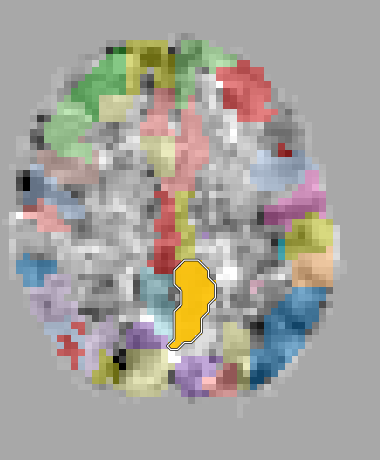
\includegraphics[height=0.84cm]{Img/pipeline_schaefer_rois_thumb.png}};

\node[panel=naranjapaper, minimum width=2.95cm] (series) at (3.15,1.72) {};
\node[title=naranjapaper] at (3.15,2.86) {Series temporales ROI};
\node[font=\scriptsize] at (3.15,2.42) {$\mathbf{X}\in\mathbb{R}^{T\times100}$};
\node[card=naranjapaper, minimum width=2.40cm, minimum height=1.28cm, inner sep=1pt] at (3.15,1.54) {};
\node at (3.15,1.54) {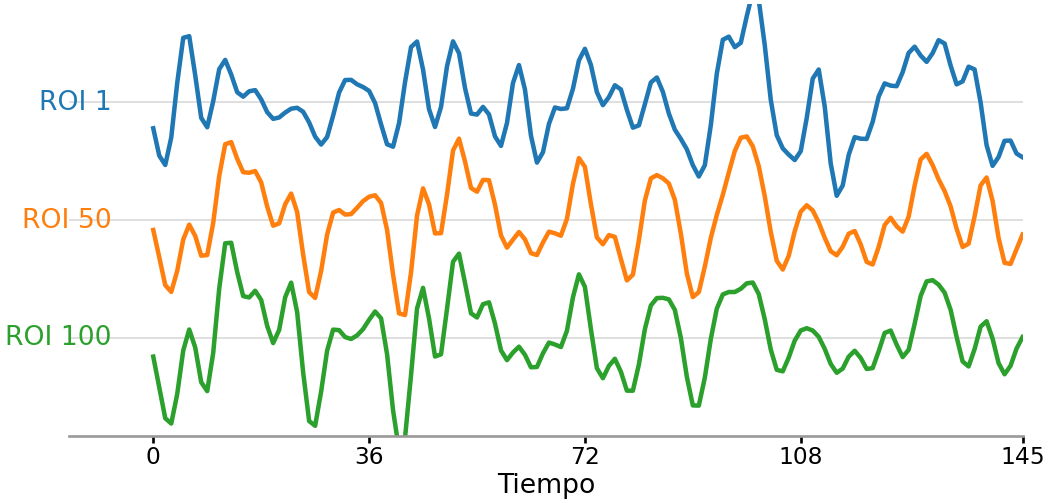
\includegraphics[width=2.25cm]{Img/pipeline_real_roi_series.png}};
\node[tinylabel] at (3.15,0.45) {se\~nales regionales z-score};

\node[panel=moradopaper, minimum width=3.35cm] (conect) at (6.65,1.72) {};
\node[title=moradopaper] at (6.65,2.88) {Estimaci\'on\\de conectividad};
\draw[dashed, draw=moradopaper!40, line width=0.60pt] (6.65,2.47) -- (6.65,0.86);
\node[font=\tiny\bfseries, text=azulpaper!75!black] at (5.88,2.30) {Asociativos};
\node[font=\tiny\bfseries, text=verdepaper!70!black, align=center] at (7.44,2.30) {Causal\\exploratorio};
\node[card=azulpaper, minimum width=1.28cm, minimum height=0.40cm] at (5.94,1.90) {Correlaci\'on};
\node[card=azulpaper, minimum width=1.28cm, minimum height=0.40cm] at (5.94,1.35) {Graphical\\Lasso};
\node[card=verdepaper, minimum width=1.28cm, minimum height=0.44cm] at (7.43,1.62) {LiNGAM};
\node[tinylabel] at (6.65,0.50) {matriz $100\times100$ por sujeto};

\node[panel=doradopaper, minimum width=3.02cm] (comparacion) at (10.15,1.72) {};
\node[title=doradopaper] at (10.15,2.88) {Comparaci\'on\\TEA y controles};
\node[tightcard=doradopaper, minimum width=2.28cm, minimum height=0.30cm] at (10.15,2.12) {Promedio controles};
\node[tightcard=doradopaper, minimum width=2.28cm, minimum height=0.30cm] at (10.15,1.66) {Promedio TEA};
\node[tightcard=doradopaper, minimum width=2.28cm, minimum height=0.40cm] at (10.15,1.16) {Diferencia\\TEA--controles};
\node[tightcard=doradopaper, minimum width=2.28cm, minimum height=0.30cm] at (10.15,0.63) {Conexiones top-20};
\node[tinylabel] at (10.15,0.28) {resumen visual descriptivo};

\node[panel=verdepaper, minimum width=2.75cm] (visual) at (13.35,1.72) {};
\node[title=verdepaper] at (13.35,2.86) {Visualizaci\'on};
\node[card=verdepaper, minimum width=2.00cm, minimum height=0.34cm] at (13.35,2.26) {Matrices promedio};
\node[card=verdepaper, minimum width=2.00cm, minimum height=0.34cm] at (13.35,1.70) {Mapas de diferencia};
\node[card=verdepaper, minimum width=2.00cm, minimum height=0.34cm] at (13.35,1.14) {Conectomas top-20};
\node[tinylabel] at (13.35,0.54) {resultados descriptivos};

% Clasificacion
\node[softpanel=grisproy, minimum width=8.85cm, minimum height=1.65cm] (posterior) at (7.55,-1.46) {};
\node[font=\bfseries\scriptsize, text=grisproy!85!black] at (7.55,-0.78)
    {Clasificaci\'on supervisada};
\node[mutedcard=grisproy, minimum width=1.60cm, minimum height=0.44cm] (vec) at (4.55,-1.48)
    {Vectorizaci\'on};
\node[mutedcard=grisproy, minimum width=1.86cm, minimum height=0.44cm] (clf) at (7.55,-1.48)
    {SVM RBF /\\Random Forest};
\node[mutedcard=grisproy, minimum width=2.45cm, minimum height=0.44cm] (met) at (10.55,-1.48)
    {Balanced accuracy, AUC};
\node[tinylabel] at (10.55,-2.00) {IC95\%, sensibilidad y especificidad};

% Flechas del flujo principal
\draw[flow] (1.37,1.72) -- (1.66,1.72);
\draw[flow] (4.68,1.72) -- (4.92,1.72);
\draw[flow] (8.38,1.72) -- (8.62,1.72);
\draw[flow] (11.70,1.72) -- (11.92,1.72);

% Flechas de la etapa preliminar
\draw[dashed, line width=0.80pt, draw=gray!50] (6.65,0.12) -- (6.65,-0.42) -| (4.55,-0.66);
\draw[prelim] (5.40,-1.48) -- (6.62,-1.48);
\draw[prelim] (8.48,-1.48) -- (9.30,-1.48);

\end{tikzpicture}%
}

\shorthandon{>} % restaurar babel
\caption[Pipeline general del an\'alisis de conectividad]{\textit{Pipeline general. El flujo resume la entrada de datos rs-fMRI de ABIDE I, la parcelación con Schaefer 100 ROIs, la extracción de series temporales, la estimación mediante correlación de Pearson, Graphical Lasso y LiNGAM, la visualización de matrices y conexiones destacadas, y la evaluación de clasificación con SVM y Random Forest.}}
\label{fig:pipeline_general}
\end{figure}

\rmfamily
\fontsize{9}{11}\selectfont
\setlength{\parskip}{5pt}
\justify

\begin{multicols}{2}

% -------------------------------------------------------
\seccionArticulo{Resultados}

La cohorte final incluyó 723 sujetos de ABIDE I: 329 TEA y 394 controles,
distribuidos en 17 sitios. Los resultados se organizan en torno a las salidas
principales del pipeline: clasificación supervisada, matrices de conectividad
estimadas mediante Pearson, Graphical Lasso y LiNGAM, y conexiones destacadas
por diferencias TEA--controles.

% -------------------------------------------------------
\subseccionArticulo{Clasificación supervisada}

La clasificación se utilizó para evaluar si las representaciones de conectividad
contenían información discriminativa entre TEA y controles. Se evaluaron los
seis pares método-clasificador: Pearson, Graphical Lasso y LiNGAM, cada uno
combinado con SVM y Random Forest.

La Tabla \ref{tab:clasificacion} incorpora \textit{balanced accuracy}, AUC,
\textit{recall}, especificidad y \textit{F1-score}. Los intervalos de confianza
del 95\% para \textit{balanced accuracy} y AUC se obtuvieron con 2000 réplicas
de \textit{bootstrap} por sitio. Pearson con SVM presentó la mayor
\textit{balanced accuracy}: 0{,}640 (IC95\%: 0{,}589--0{,}675). Graphical Lasso
con Random Forest obtuvo el mayor AUC: 0{,}686 (IC95\%: 0{,}632--0{,}738),
aunque con menor \textit{recall}. LiNGAM obtuvo \textit{balanced accuracy} de
0{,}499 con SVM y 0{,}461 con Random Forest, además de AUC inferiores a 0{,}45.

Estos resultados indican desempeño predictivo moderado para Pearson con SVM y
Graphical Lasso con Random Forest, sin respaldar una ventaja predictiva de la
representación causal exploratoria de LiNGAM bajo esta configuración. La Figura
\ref{fig:roc} muestra las curvas ROC correspondientes.

\end{multicols}

\begin{table}[H]
\centering
\scriptsize
\setlength{\tabcolsep}{2pt}
\begin{tabular}{llrrrrr}
\toprule
Método & Clasificador & Balanced accuracy (IC95\%) & AUC (IC95\%) & Recall & Especificidad & F1 \\
\midrule
Pearson & SVM & 0{,}640 (0{,}589--0{,}675) & 0{,}674 (0{,}622--0{,}721) & 0{,}559 & 0{,}721 & 0{,}591 \\
Pearson & Random Forest & 0{,}595 (0{,}557--0{,}625) & 0{,}650 (0{,}604--0{,}693) & 0{,}401 & 0{,}789 & 0{,}485 \\
Graphical Lasso & SVM & 0{,}540 (0{,}507--0{,}576) & 0{,}593 (0{,}549--0{,}661) & 0{,}550 & 0{,}530 & 0{,}521 \\
Graphical Lasso & Random Forest & 0{,}586 (0{,}556--0{,}626) & 0{,}686 (0{,}632--0{,}738) & 0{,}350 & 0{,}822 & 0{,}447 \\
LiNGAM & SVM & 0{,}499 (0{,}487--0{,}508) & 0{,}443 (0{,}403--0{,}489) & 0{,}052 & 0{,}947 & 0{,}093 \\
LiNGAM & Random Forest & 0{,}461 (0{,}445--0{,}488) & 0{,}438 (0{,}415--0{,}468) & 0{,}207 & 0{,}716 & 0{,}267 \\
\bottomrule
\end{tabular}
\caption{\textit{Clasificación de TEA y controles mediante predicciones out-of-fold. Los IC95\% se obtuvieron con 2000 réplicas de bootstrap por sitio.}}
\label{tab:clasificacion}
\end{table}

\begin{figure}[H]
    \centering
    \includegraphics[width=0.82\textwidth]{../resultados/pipeline_versiones9/figures/curvas_roc_tea_controles.png}
    \caption{\textit{Curvas ROC para la clasificación de TEA y controles.}}
    \label{fig:roc}
\end{figure}

\begin{multicols}{2}

% -------------------------------------------------------
\subseccionArticulo{Matrices de conectividad de Pearson y Graphical Lasso}

Las Figuras \ref{fig:pearson_panel} y \ref{fig:lasso_panel} muestran las
matrices promedio por grupo y la diferencia TEA $-$ controles para los dos
métodos asociativos. Las regiones se ordenan según las siete redes funcionales
del atlas Schaefer 100 y las matrices completas de 100 ROIs se presentan sin
filtrado estadístico, con el fin de mostrar el patrón global producido por cada
estimador.

Pearson produjo una matriz densa de conectividad funcional bivariada,
consistente con una medida de sincronía lineal entre pares de ROIs. Graphical
Lasso produjo una matriz regularizada de menor magnitud y más dispersa,
interpretable como correlación parcial normalizada derivada de la matriz de
precisión estimada con $\alpha=0{,}5$. Por tanto, Pearson resume asociaciones
lineales directas e indirectas, mientras que Graphical Lasso resalta
dependencias condicionales más selectivas.

La Tabla \ref{tab:metricas_sujeto} y la Figura \ref{fig:metricas_sujeto}
complementan la lectura visual con magnitud absoluta media y esparsidad por
sujeto. Estas métricas son descriptivas y no reemplazan el análisis por
conexión. En promedio, Pearson mostró una magnitud absoluta media muy similar
entre grupos, mientras que Graphical Lasso presentó valores de menor escala y
alta esparsidad en ambos grupos.

\end{multicols}

\begin{figure}[H]
    \centering
    \includegraphics[width=0.98\textwidth]{../resultados/pipeline_versiones9/figures/correlacion_control_tea_diff_panel.png}
    \caption{\textit{Matrices completas de 100 ROIs: promedio y diferencia TEA $-$ controles para correlación de Pearson, ordenadas por redes funcionales.}}
    \label{fig:pearson_panel}
\end{figure}

\begin{figure}[H]
    \centering
    \includegraphics[width=0.98\textwidth]{../resultados/pipeline_versiones9/figures/lasso_control_tea_diff_panel.png}
    \caption{\textit{Matrices completas de 100 ROIs: promedio y diferencia TEA $-$ controles para Graphical Lasso, ordenadas por redes funcionales.}}
    \label{fig:lasso_panel}
\end{figure}

\begin{table}[H]
\centering
\small
\begin{tabular}{llrrr}
\toprule
Método & Métrica & Controles & TEA & Diferencia TEA $-$ controles \\
\midrule
Pearson & Magnitud & 0{,}3465 (0{,}1003) & 0{,}3448 (0{,}1015) & $-0{,}0017$ \\
Pearson & Esparsidad & 0{,}0015 (0{,}0024) & 0{,}0016 (0{,}0020) & 0{,}0001 \\
Graphical Lasso & Magnitud & 0{,}0076 (0{,}0012) & 0{,}0075 (0{,}0013) & $-0{,}0001$ \\
Graphical Lasso & Esparsidad & 0{,}8891 (0{,}0340) & 0{,}8904 (0{,}0353) & 0{,}0013 \\
\bottomrule
\end{tabular}
\caption{\textit{Magnitud absoluta media y esparsidad calculadas por sujeto. Los valores grupales son media (DE); la diferencia corresponde a TEA menos controles.}}
\label{tab:metricas_sujeto}
\end{table}

\begin{figure}[H]
    \centering
    \includegraphics[width=0.84\textwidth]{../resultados/pipeline_versiones9/figures/distribuciones_conectividad_por_sujeto.png}
    \caption{\textit{Distribuciones por sujeto de magnitud absoluta media y esparsidad para Pearson y Graphical Lasso.}}
    \label{fig:metricas_sujeto}
\end{figure}

% -------------------------------------------------------
\begin{multicols}{2}
\subseccionArticulo{Representación causal - \texorpdfstring{\mbox{LiNGAM}}{LiNGAM}}

LiNGAM se interpreta como la representación causal exploratoria dentro del
diseño metodológico del estudio. La Figura \ref{fig:lingam_panel} muestra las matrices promedio y la
diferencia TEA $-$ controles para pesos orientados normalizados por sujeto. A
diferencia de Pearson y Graphical Lasso, la matriz de LiNGAM no es simétrica y
conserva el sentido de las aristas en las salidas tabulares.

La Figura \ref{fig:top20_lingam} resume las 20 conexiones de LiNGAM con mayor
diferencia absoluta entre grupos. Estas aristas se interpretan como patrones
descriptivos orientados bajo los supuestos de LiNGAM. Debido a la
naturaleza indirecta de la señal BOLD, la respuesta hemodinámica, la posible
presencia de confundentes no observados y la normalización de pesos dentro de
cada sujeto, su lectura debe mantenerse prudente por las limitaciones de la
señal BOLD y los supuestos del método.

\end{multicols}

\begin{figure}[H]
    \centering
    \includegraphics[width=0.98\textwidth]{../resultados/pipeline_versiones9/figures/lingam_control_tea_diff_panel.png}
    \caption{\textit{Matrices completas de 100 ROIs: promedio y diferencia TEA $-$ controles para LiNGAM. Los valores corresponden a pesos orientados relativos normalizados dentro de cada sujeto.}}
    \label{fig:lingam_panel}
\end{figure}

\begin{figure}[H]
    \centering
    \includegraphics[width=0.98\textwidth]{../resultados/pipeline_versiones9/figures/lingam_control_tea_diff_top20_connectomes_panel.png}
    \caption{\textit{Conectomas con 20 conexiones para LiNGAM. La proyección representa la ubicación de las aristas; el sentido de la relación se conserva en las tablas de resultados.}}
    \label{fig:top20_lingam}
\end{figure}

\begin{multicols}{2}
% -------------------------------------------------------
\subseccionArticulo{Conexiones destacadas y diferencias TEA--controles}

Las Figuras \ref{fig:top20_pearson}, \ref{fig:top20_lasso} y
\ref{fig:top20_lingam} muestran conectomas con las 20 conexiones de mayor
diferencia absoluta entre TEA y controles por método. En Pearson, las
diferencias destacadas incluyeron pares Default--Control/frontoparietal,
Default--Default y DorsAttn--Default. En Graphical Lasso, las diferencias fueron
más focales y se concentraron en pares Default--Default, además de conexiones
somatomotoras, visuales y de saliencia/atención ventral. En LiNGAM, las
conexiones destacadas incluyeron pares Visual--Control, Default--Default,
Visual--Visual y saliencia/atención ventral, manteniendo la orientación en las
tablas de resultados.

Como salida complementaria ya calculada, la Figura \ref{fig:nbs_componentes}
presenta matrices NBS para Pearson y Graphical Lasso. Este análisis no forma
parte del flujo central de estimación y clasificación, sino que se conserva como
apoyo descriptivo para visualizar subredes de diferencias TEA--controles.

\end{multicols}

\begin{figure}[H]
    \centering
    \includegraphics[width=0.98\textwidth]{../resultados/pipeline_versiones9/figures/correlacion_control_tea_diff_top20_connectomes_panel.png}
    \caption{\textit{Conectomas con 20 conexiones para Pearson: controles, TEA y diferencia TEA $-$ controles.}}
    \label{fig:top20_pearson}
\end{figure}

\begin{figure}[H]
    \centering
    \includegraphics[width=0.98\textwidth]{../resultados/pipeline_versiones9/figures/lasso_control_tea_diff_top20_connectomes_panel.png}
    \caption{\textit{Conectomas con 20 conexiones para Graphical Lasso: controles, TEA y diferencia TEA $-$ controles.}}
    \label{fig:top20_lasso}
\end{figure}


\begin{multicols}{2}
% -------------------------------------------------------
\seccionArticulo{Discusión}

\subseccionArticulo{Desempeño de clasificación}

La clasificación supervisada se utilizó como una evaluación del poder
discriminativo de las representaciones de conectividad, no como una prueba
diagnóstica. La combinación con mejor \textit{balanced accuracy} fue Pearson
con SVM (0{,}640; IC95\% 0{,}589--0{,}675), acompañada de un AUC de 0{,}674,
un \textit{recall} de 0{,}559 y una especificidad de 0{,}721. Graphical Lasso
con Random Forest alcanzó el AUC más alto (0{,}686), pero con menor sensibilidad
(0{,}350) y mayor especificidad (0{,}822), lo que indica un perfil más
conservador para detectar sujetos TEA.

Los resultados de LiNGAM fueron inferiores en esta tarea predictiva. En
particular, LiNGAM con SVM mostró \textit{balanced accuracy} cercana al azar
(0{,}499) y un \textit{recall} muy bajo (0{,}052), aunque con especificidad alta
(0{,}947). Por tanto, bajo esta configuración y con las características
vectorizadas disponibles, la representación causal exploratoria no añadió una
ventaja predictiva frente a Pearson o Graphical Lasso. Estos desempeños son
moderados y deben interpretarse como comparación metodológica dentro de ABIDE I,
sin atribuirles validez clínica directa.

\subseccionArticulo{Diferencias de conectividad y redes destacadas}

El orden de los resultados muestra primero el desempeño predictivo y luego las
estructuras de conectividad que sostienen la interpretación. Pearson produjo
matrices asociativas densas, simétricas por definición matemática, y sus
conexiones destacadas incluyeron pares Default--Control/frontoparietal,
Default--Default y DorsAttn--Default. Graphical Lasso generó una lectura más
dispersa de dependencias condicionales, con diferencias concentradas en pares
Default--Default y en conexiones somatomotoras, visuales y de
saliencia/atención ventral.

LiNGAM aportó matrices orientadas bajo un modelo causal exploratorio. Sus
conexiones destacadas incluyeron pares Visual--Control, Default--Default,
Visual--Visual y saliencia/atención ventral. Esta orientación no debe leerse
como demostración de causalidad fisiológica, sino como una representación
estadística condicionada por los supuestos del método y por las limitaciones de
la señal BOLD. Las matrices NBS calculadas para Pearson y Graphical Lasso se
mantienen como apoyo descriptivo complementario para visualizar subredes, no
como eje principal del pipeline.

\subseccionArticulo{Relación de los hallazgos con la literatura}

Los resultados se relacionan con estudios que han descrito alteraciones
distribuidas de conectividad funcional en TEA usando rs-fMRI y cohortes
multicéntricas como ABIDE \cite{diMartino2014autism,nielsen2013multisite}.
La participación de redes Default, Control/frontoparietal, atención dorsal,
saliencia, somatomotora y visual es compatible con una lectura de reorganización
funcional amplia, previamente discutida en revisiones y trabajos sobre TEA
\cite{uddin2013reconceptualizing,hull2017review}. No obstante, el patrón no
debe resumirse como hiperconectividad o hipoconectividad global, porque los
signos variaron según conexión, método y forma de estimación.

El contraste entre Pearson y Graphical Lasso también coincide con la diferencia
conceptual entre asociación bivariada y dependencia condicional regularizada
\cite{smith2013functional,friedman2008sparse}. Pearson tiende a preservar
relaciones densas entre señales regionales, mientras que Graphical Lasso busca
una estructura más esparsa a partir de la matriz de precisión. La Tabla
\ref{tab:hallazgos_literatura} resume la relación entre los hallazgos
descriptivos, las redes implicadas y el alcance prudente de su interpretación.

\end{multicols}

\begin{table}[H]
\centering
\footnotesize
\setlength{\tabcolsep}{3pt}
\renewcommand{\arraystretch}{1.08}
\begin{tabular}{>{\raggedright\arraybackslash}p{0.22\linewidth} >{\raggedright\arraybackslash}p{0.23\linewidth} >{\raggedright\arraybackslash}p{0.18\linewidth} >{\raggedright\arraybackslash}p{0.25\linewidth}}
\toprule
Hallazgo del trabajo & Red/región involucrada & Signo o alcance & Relación con la literatura \\
\midrule
Clasificación supervisada & Representaciones vectorizadas de Pearson, Graphical Lasso y LiNGAM & Pearson--SVM obtuvo la mayor balanced accuracy; Graphical Lasso--Random Forest obtuvo el mayor AUC & Compatible con reportes de clasificación moderada en ABIDE; no constituye biomarcador clínico \\
Diferencias descriptivas top-20 & Pearson: Default--Control y Default--Default; Graphical Lasso: Default--Default y redes sensoriomotoras/visuales & Signos mixtos según conexión & Sugiere heterogeneidad de patrones, sin reducir el resultado a hiper o hipoconectividad global \\
LiNGAM como representación causal exploratoria & Conexiones de LiNGAM en redes Visual, Default, SalVentAttn y Control, entre otras & Lectura cautelosa & Limitado por señal BOLD, normalización por sujeto y supuestos no verificados; no demuestra un mecanismo cerebral por sí solo \\
\bottomrule
\end{tabular}
\caption{\textit{Relación entre los principales hallazgos y la literatura. La tabla resume resultados reales del análisis y su alcance interpretativo; no propone biomarcadores clínicos ni mecanismos fisiológicos demostrados.}}
\label{tab:hallazgos_literatura}
\end{table}

\begin{multicols}{2}

\subseccionArticulo{Aporte y límites de LiNGAM}

LiNGAM es el método causal del contraste metodológico, pero su uso en este
trabajo se define explícitamente como exploratorio. Su aporte principal es
producir una matriz orientada que permite preguntar si la información extraída
por un modelo causal lineal difiere de las representaciones asociativas de
Pearson y Graphical Lasso. En los resultados obtenidos, esta representación no
mejoró la clasificación supervisada ni permitió identificar un mecanismo
neurofisiológico demostrado.

La cautela es necesaria porque LiNGAM asume linealidad, aciclicidad,
independencia de errores y no gaussianidad, condiciones que no fueron
verificadas exhaustivamente en esta cohorte. Además, la señal BOLD es una
medida hemodinámica indirecta, con baja resolución temporal y posibles
desfases regionales \cite{ogawa1990brain,logothetis2001neurophysiological,
buxton1998dynamics}. Por ello, la orientación estimada por LiNGAM se interpreta
como una hipótesis estadística dentro del modelo, no como causalidad fisiológica
probada.

\subseccionArticulo{Limitaciones metodológicas}

La cohorte proviene de ABIDE I, una base multicéntrica con heterogeneidad en
sitios, protocolos de adquisición, calidad de imagen, características
demográficas y movimiento residual. Estos factores pueden actuar como
confundentes si afectan simultáneamente las señales BOLD o la composición de los
grupos. En este trabajo se describen como limitaciones metodológicas y no como
ejes centrales del análisis \cite{power2012spurious,ciric2017benchmarking}.

También deben considerarse el CI faltante en parte de la muestra, la ausencia
de una cohorte externa, la validación no anidada de hiperparámetros, la
validación técnica piloto del parámetro $\alpha$ de Graphical Lasso y el uso de
146 puntos temporales como criterio operacional mínimo, útil para mantener
$T>K$ con 100 ROIs, pero insuficiente por sí solo para garantizar estabilidad
estadística. Los componentes NBS dependen del umbral primario $|t|\geq3{,}1$ y
se conservaron como análisis complementario de subredes
\cite{zalesky2010network}. En conjunto, estas limitaciones impiden presentar los
resultados como biomarcador clínico o prueba fisiológica definitiva.


% -------------------------------------------------------
\seccionArticulo{Conclusión}

Se implementó un pipeline reproducible con datos ABIDE I, atlas Schaefer 100,
extracción de señales BOLD regionales, estimación de matrices individuales,
vectorización y clasificación supervisada. Se contrastaron tres métodos
principales de conectividad:
correlación de Pearson, Graphical Lasso y LiNGAM.

Pearson y Graphical Lasso permitieron caracterizar patrones asociativos de
conectividad con lecturas complementarias: Pearson como asociación bivariada y
Graphical Lasso como dependencia condicional regularizada. Las matrices,
conectomas top-20 y análisis complementarios sugirieron diferencias
distribuidas en redes Default, Control/frontoparietal, atención, saliencia,
somatomotoras y visuales. Estos hallazgos son compatibles con alteraciones de
conectividad funcional descritas en TEA, aunque no constituyen un patrón único
ni específico.

LiNGAM se aplicó como representación causal exploratoria. Bajo esta configuración, no
mostró una ventaja predictiva frente a Pearson y Graphical Lasso, por lo que
sus resultados deben interpretarse con cautela debido a las limitaciones de la
señal BOLD y a los supuestos del método. La clasificación supervisada se
mantuvo como evaluación complementaria del poder discriminativo de las matrices:
Pearson con SVM y Graphical Lasso con Random Forest ofrecieron los mejores
desempeños preliminares, pero estos fueron moderados.

El aporte principal del trabajo es metodológico, comparativo e interpretativo.
Las conclusiones se restringen a la cohorte analizada y deben leerse con
cautela por la heterogeneidad entre sitios, movimiento residual, datos faltantes
de cociente intelectual, ausencia de una cohorte independiente, validación no
anidada, elección del umbral NBS como análisis complementario y validación
técnica piloto del parámetro $\alpha$ de Graphical Lasso.
Por tanto, el estudio no propone un biomarcador clínico ni mecanismos
fisiológicos demostrados; aporta una comparación reproducible de representaciones de
conectividad cerebral en TEA.


\end{multicols}

% -------------------------------------------------------
% [MOVIDO] Las referencias permanecen al final del documento.
\bibliographystyle{IEEEtran}
\begin{multicols}{2}
\bibliography{referencias}
\end{multicols}

\end{document}
